\documentclass[aspectratio=169,10pt]{beamer}
\usetheme{Madrid}
\usecolortheme{default}

% Packages
\usepackage{graphicx}
\usepackage{booktabs}
\usepackage{tikz}
\usetikzlibrary{positioning,arrows.meta}

% Colors
\definecolor{ntublue}{RGB}{0,61,124}
\definecolor{successgreen}{RGB}{40,167,69}
\definecolor{warningyellow}{RGB}{255,193,7}
\definecolor{dangerred}{RGB}{220,53,69}

\setbeamercolor{structure}{fg=ntublue}
\setbeamercolor{block title}{bg=ntublue,fg=white}

% Reduce margins
\setbeamersize{text margin left=8mm,text margin right=8mm}

% Title Info
\title{Real Estate App Development \& Recommendation}
\subtitle{FYP Progress Report}
\author{Wang Yangming}
\institute{Nanyang Technological University}
\date{\today}

\begin{document}

% ===== Title Slide =====
\begin{frame}
    \titlepage
\end{frame}

% ===== Outline =====
\begin{frame}{Outline}
    \tableofcontents
\end{frame}

% ===== Section 1 =====
\section{Recap: Previous Progress}

\begin{frame}{Recap: Winter Break Progress}
    \begin{columns}[T]
        \column{0.48\textwidth}
        \textbf{Completed:}
        \begin{itemize}
            \item Reliability Verification
            \item Parallelism Troubleshooting
            \item Operational Pivot to single-thread/proxy
            \item Pipeline Development (initial design)
        \end{itemize}
        
        \column{0.48\textwidth}
        \textbf{Planned Future Work:}
        \begin{itemize}
            \item Test Cron Job's Reliability
            \item Design Merging Logic (multi-site)
            \item Design Merging Logic (Gov data)
            \item Backend Development
        \end{itemize}
    \end{columns}
\end{frame}

% ===== Section 2 =====
\section{Progress: Past Two Weeks}

\begin{frame}{Overview: Tasks Completed}
    \begin{table}[]
        \centering
        \large
        \begin{tabular}{lcc}
            \toprule
            \textbf{Task} & \textbf{Status} & \textbf{Completion} \\
            \midrule
            Multi-Platform Scrapers & \textcolor{successgreen}{Operational} & 90\% \\
            Data Merging Pipeline & \textcolor{successgreen}{Operational} & 90\% \\
            Database Schema Design & \textcolor{successgreen}{Complete} & 100\% \\
            Cron Job Setup & \textcolor{warningyellow}{Configured} & 90\% \\
            \bottomrule
        \end{tabular}
    \end{table}
    
    \vspace{0.5cm}
    
    \begin{center}
    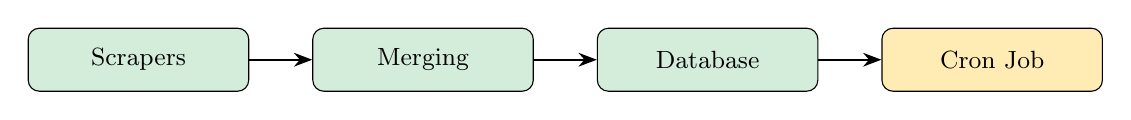
\begin{tikzpicture}[
        node distance=0.8cm,
        box/.style={draw, rounded corners, minimum width=2.8cm, minimum height=0.8cm, font=\small}
    ]
        \node[box, fill=successgreen!20] (s1) {Scrapers};
        \node[box, fill=successgreen!20, right=of s1] (s2) {Merging};
        \node[box, fill=successgreen!20, right=of s2] (s3) {Database};
        \node[box, fill=warningyellow!30, right=of s3] (s4) {Cron Job};
        
        \draw[-{Stealth}, thick] (s1) -- (s2);
        \draw[-{Stealth}, thick] (s2) -- (s3);
        \draw[-{Stealth}, thick] (s3) -- (s4);
    \end{tikzpicture}
    \end{center}
\end{frame}

\begin{frame}{1. Multi-Platform Scrapers}
    \textbf{Coverage: 4 Major Singapore Property Portals}
    
    \vspace{0.4cm}
    
    \begin{columns}[T]
        \column{0.48\textwidth}
        \textbf{PropertyGuru}
        \begin{itemize}
            \item Tech: Requests + Proxy API
            \item Data: Sale \& Rental listings
            \item Feature: Incremental update, auto-cleanup
        \end{itemize}
        
        \vspace{0.3cm}
        
        \textbf{99.co}
        \begin{itemize}
            \item Tech: Playwright (headless)
            \item Data: Sale \& Rental listings
            \item Feature: Retry logic, pagination
        \end{itemize}
        
        \column{0.48\textwidth}
        \textbf{EdgeProp}
        \begin{itemize}
            \item Tech: Playwright (headless)
            \item Data: HDB / Condo / Landed
            \item Feature: Debug HTML snapshots
        \end{itemize}
        
        \vspace{0.3cm}
        
        \textbf{SRX}
        \begin{itemize}
            \item Tech: Playwright (headless)
            \item Data: Sale \& Rental (by town)
            \item Feature: Concurrent crawling, CSV backup
        \end{itemize}
    \end{columns}
\end{frame}

\begin{frame}{2. Data Merging Pipeline (1/2)}
    \textbf{Implementation: \texttt{pipeline/aggregate.py}}
    
    \vspace{0.4cm}
    
    \begin{columns}[T]
        \column{0.48\textwidth}
        \textbf{Standardization Functions:}
        \begin{itemize}
            \item \texttt{normalize\_propertyguru()}
            \item \texttt{normalize\_99co()}
            \item \texttt{normalize\_edgeprop()}
            \item \texttt{normalize\_srx()}
        \end{itemize}
        
        \column{0.48\textwidth}
        \textbf{Data Cleansing:}
        \begin{itemize}
            \item \texttt{clean\_price()} $\rightarrow$ numeric
            \item \texttt{clean\_sqft()} $\rightarrow$ numeric
            \item \texttt{clean\_tenure()} $\rightarrow$ unified
            \item \texttt{clean\_property\_type()}
        \end{itemize}
    \end{columns}
\end{frame}

\begin{frame}{2. Data Merging Pipeline (2/2)}
    \begin{columns}[T]
        \column{0.48\textwidth}
        \textbf{Deduplication Logic:}
        \begin{itemize}
            \item Composite Key:
            \begin{itemize}
                \item Normalized Address
                \item Beds + Baths + Sqft
            \end{itemize}
            \item Source Priority: PropertyGuru first
        \end{itemize}
        
        \column{0.48\textwidth}
        \textbf{Price Format Unification:}
        \begin{itemize}
            \item Sale: \texttt{S\$ 1,234,567}
            \item Rental: \texttt{S\$ 3,500 /mo}
            \item PSF: \texttt{S\$ 1,234.56 psf}
        \end{itemize}
    \end{columns}
    
    \vspace{0.5cm}
    
    \begin{block}{Output}
        Unified \texttt{aggregated\_listings.csv} with consistent schema across all platforms
    \end{block}
\end{frame}

\begin{frame}{3. Database Architecture}
    \begin{columns}[T]
        \column{0.45\textwidth}
        \textbf{Dual Database Support:}
        \begin{itemize}
            \item PostgreSQL (production)
            \item SQLite (local dev)
        \end{itemize}
        
        \vspace{0.3cm}
        
        \textbf{Schema Design:}
        \begin{itemize}
            \item \texttt{agents} table
            \item \texttt{listings} table
            \item FK: \texttt{agent\_id}
            \item Unique: \texttt{url}
        \end{itemize}
        
        \column{0.50\textwidth}
        \textbf{Key Fields in \texttt{listings}:}
        \begin{itemize}
            \item title, address
            \item price (numeric), display\_price
            \item psf (numeric), display\_psf
            \item beds, baths, sqft
            \item property\_type, tenure
            \item source, buy\_rent
            \item created\_at, updated\_at
        \end{itemize}
    \end{columns}
\end{frame}

\begin{frame}{4. Cron Job Configuration}
    \textbf{Automated Scheduling (Ready for Deployment):}
    
    \vspace{0.5cm}
    
    \begin{table}[]
        \centering
        \begin{tabular}{lll}
            \toprule
            \textbf{Task} & \textbf{Schedule} & \textbf{Script} \\
            \midrule
            Daily Incremental Update & 2:00 AM daily & \texttt{run\_daily.py} \\
            Weekly Cleanup & 3:00 AM Monday & \texttt{run\_cleanup.py} \\
            Retry Failed Records & On-demand & \texttt{run\_retry.py} \\
            \bottomrule
        \end{tabular}
    \end{table}
    
    \vspace{0.5cm}
    
    \textbf{Crontab Example:}
    
    \vspace{0.2cm}
    
    {\small\texttt{0 2 * * * python run\_daily.py >> daily.log 2>\&1}}
    
    {\small\texttt{0 3 * * 1 python run\_cleanup.py >> cleanup.log 2>\&1}}
\end{frame}

% ===== Section 3 =====
\section{Data Flow}

\begin{frame}{Data Flow Architecture}
    \begin{center}
    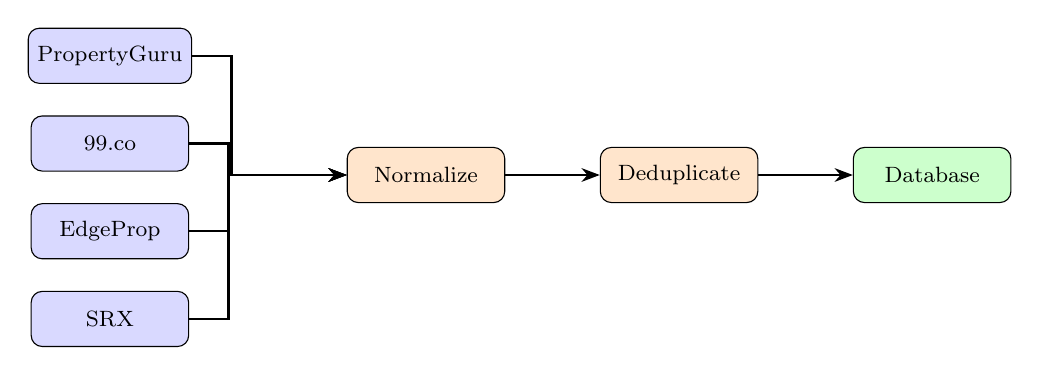
\begin{tikzpicture}[
        node distance=1.2cm,
        box/.style={draw, rounded corners, minimum width=2cm, minimum height=0.7cm, font=\footnotesize},
        >=Stealth
    ]
        % Source nodes
        \node[box, fill=blue!15] (pg) {PropertyGuru};
        \node[box, fill=blue!15, below=0.4cm of pg] (co) {99.co};
        \node[box, fill=blue!15, below=0.4cm of co] (ep) {EdgeProp};
        \node[box, fill=blue!15, below=0.4cm of ep] (srx) {SRX};
        
        % Process nodes
        \node[box, fill=orange!20, right=2cm of co, yshift=-0.4cm] (norm) {Normalize};
        \node[box, fill=orange!20, right=1.2cm of norm] (dedup) {Deduplicate};
        \node[box, fill=green!20, right=1.2cm of dedup] (db) {Database};
        
        % Arrows
        \draw[->, thick] (pg.east) -- ++(0.5,0) |- (norm.west);
        \draw[->, thick] (co.east) -- ++(0.5,0) |- (norm.west);
        \draw[->, thick] (ep.east) -- ++(0.5,0) |- (norm.west);
        \draw[->, thick] (srx.east) -- ++(0.5,0) |- (norm.west);
        \draw[->, thick] (norm) -- (dedup);
        \draw[->, thick] (dedup) -- (db);
    \end{tikzpicture}
    \end{center}
    
    \vspace{0.4cm}
    
    \begin{itemize}
        \item \textbf{Input}: 4 platforms $\times$ 2 categories (Sale/Rent)
        \item \textbf{Output}: Unified CSV + PostgreSQL/SQLite database
    \end{itemize}
\end{frame}

% ===== Section 4 =====
\section{Next Steps}

\begin{frame}{Future Work}
    \begin{columns}[T]
        \column{0.48\textwidth}
        \textbf{Short-term (Next 2 Weeks):}
        \begin{enumerate}
            \item Integrate Government Data
            \begin{itemize}
                \item HDB info from data.gov.sg
                \item URA transaction records
            \end{itemize}
            \item Backend API Development
            \begin{itemize}
                \item FastAPI REST API
                \item Search \& Filter endpoints
            \end{itemize}
        \end{enumerate}
        
        \column{0.48\textwidth}
        \textbf{Medium-term:}
        \begin{enumerate}
            \setcounter{enumi}{2}
            \item Recommendation System
            \begin{itemize}
                \item Multi-factor analysis
                \item Price prediction model
            \end{itemize}
            \item Frontend Development
            \begin{itemize}
                \item Web/Mobile interface
            \end{itemize}
        \end{enumerate}
    \end{columns}
    
    \vspace{0.6cm}
    
    \begin{center}
    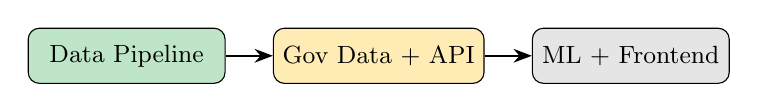
\begin{tikzpicture}[
        node distance=0.6cm,
        box/.style={draw, rounded corners, minimum width=2.5cm, minimum height=0.7cm, font=\small}
    ]
        \node[box, fill=successgreen!30] (done) {Data Pipeline};
        \node[box, fill=warningyellow!30, right=of done] (curr) {Gov Data + API};
        \node[box, fill=gray!20, right=of curr] (next) {ML + Frontend};
        
        \draw[-{Stealth}, thick] (done) -- (curr);
        \draw[-{Stealth}, thick] (curr) -- (next);
    \end{tikzpicture}
    \end{center}
\end{frame}

% ===== Summary =====
\section{Summary}

\begin{frame}{Summary}
    \begin{block}{Key Achievements (Week 3--4)}
        \begin{itemize}
            \item Developed scrapers for 4 major Singapore property platforms
            \item Implemented data merging pipeline with standardization \& deduplication
            \item Designed dual-database schema (PostgreSQL + SQLite)
            \item Configured automated cron job scheduling for daily updates
        \end{itemize}
    \end{block}
    
    \vspace{0.3cm}
    
    \begin{block}{Next Priorities (Week 5--6)}
        \begin{itemize}
            \item Integrate government data sources (HDB, URA via data.gov.sg)
            \item Develop FastAPI backend with RESTful endpoints
        \end{itemize}
    \end{block}
\end{frame}

% ===== End =====
\begin{frame}
    \begin{center}
        \Huge Thank You!
        
        \vspace{1cm}
        
        \Large Questions?
    \end{center}
\end{frame}

\end{document}